
\chapter{Background}
\label{cha:background}
In this chapter the main topics needed to understand this work are presented. A more
detailed explanation of each topic can be found on the respective cited work.
\section{Systems}

A System as defined by the Cambridge's dictionary is ``a set of connected things
or devices that operate together''. As seen two basic properties of systems are
:
\begin{itemize}
\item they are formed by grouping smaller parts
\item the smaller parts when grouped work together to carry out a specific
  function
\end{itemize}

Usually, systems are modelled by an Input\slash Output process. The system is fed with a
set of inputs, it processes the inputs resulting on the output set, as we can see
in \autoref{fig:ioProcModel}.

\begin{figure}[H]
  \centering
  \begin{tikzpicture}
    % \node[anchor=south west,inner sep=0] (image) at (0,0) {
    %   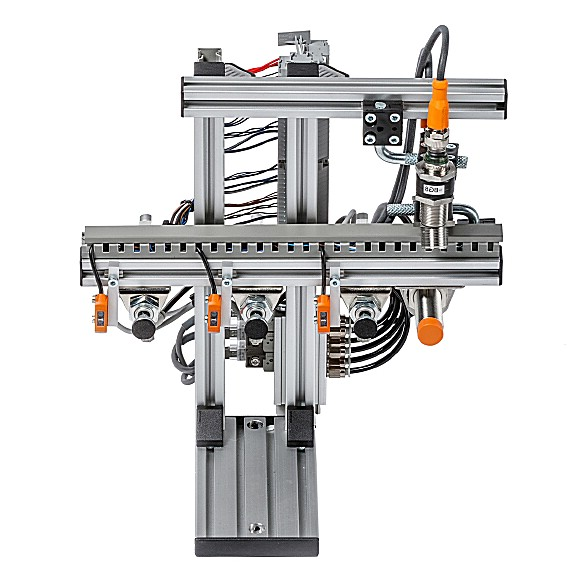
\includegraphics[trim={0 0 0 0},clip,width=8cm]{maquete/sensores/69511_3.jpg}
    % };
    % \draw[red,ultra thick,rounded corners] (0,0) rectangle (9.4,6.2);
    % \begin{scope}[x={(image.south east)},y={(image.north west)}]
        \draw[ultra thick,rounded corners] (3.5,4) rectangle (6.5,6);
        \draw (5,5) node {\textbf{Process}};
        \draw (0,5) node {\textbf{Inputs}};
        \draw[->,>=stealth, very thick] (1,4.5) -- ++ (2.5,0);
        \draw[->,>=stealth, very thick] (1,5)   -- ++ (2.5,0);
        \draw[->,>=stealth, very thick] (1,5.5) -- ++ (2.5,0);
        \draw (10,5) node {\textbf{Outputs}};
        \draw[->,>=stealth, very thick] (6.5,4.5) -- ++ (2.5,0);
        \draw[->,>=stealth, very thick] (6.5,5)   -- ++ (2.5,0);
        \draw[->,>=stealth, very thick] (6.5,5.5) -- ++ (2.5,0);
      % \end{scope}
    \end{tikzpicture}
  \caption{Input\slash Output Process model}
    \label{fig:ioProcModel}
\end{figure}

The states of the system can be continuous or discrete, and the systems can be considered as Continuous, Discrete or 
Hybrid Systems, which combine both kind of states.

The systems modelled in this work are Discrete Systems. More details about other
kinds of systems as well as examples and their analysis can be found on
\cite{oppenheim1996signals} and \cite{kalouptsidis1997signal}.
\section{Discrete Event Systems}
\label{sec:discreteEventSystems}
Discrete Systems can be driven by time or by events, i.e., the states can
change continuously with the time or instantaneously with the occurrence of events.

In this work, we are interested in the event-driven type. Some basic mathematical
formalisms, nomenclature and representations can be developed to facilitate the
understanding. Some of those will be presented in the following sections based
on \cite{cassandras2009introduction, david2005discrete,david1989grafcet}.
\section{Languages} \label{sec:automata} A language can be defined by the Merriam-Webster's dictionary as ``a systematic
means of communicating ideas or feelings by the use of conventionalized signs,
sounds, gestures, or marks having understood meanings'', and as it is defined by
this dictionary entry we pursue to communicate the complete behaviour of the
\DES. Firstly we need to define a group, or set of marks to characterise the
singular behaviour of the system. So, we define a set $\Sigma$. This set contains
all elements which combined can create a language. Again in analogy with
linguistics, each one of these marks, the events can be compared to letters,
provided that $\Sigma$ can be called an ``alphabet'', and the combination of its
events ``words''. Words are also called ``strings '' or even ``traces''.
Considering the use of the word ``string'' as the variable type used on several
programming languages used in this work, we prefer the use of the terms
``word'' and ``trace''. We can also define the empty word,
$\epsilon$, that is, a word that is not formed by any event.

The operation to form words is called concatenation. For instance,
given two events $a$ and $b$, the words $ab$ and $ba$ can be created
concatenating these two events and there is no particular reason to suppose that
$ab$ is equal to $ba$. The same goes for the words ``ten'' and ``net'', that have different meanings in English.

We can also concatenate two words to create a different one. For instance, we can take the
words $ab$ and $ba$ and create words like $abba$ and $baab$.

As we extended the definition of concatenation to words, we define $\epsilon$,
the empty word, as the identity element of concatenation: $w\epsilon = \epsilon
w = w$ for any word $w$.

Likewise, we can define the length of a word as the number of events contained
by this word. We denote the length with two vertical bars. Thus, given a word $w$ its
length is equal to $|w|$ and by definition $|\epsilon| = 0 $.

% As we know, there is a great number of human western languages, as portuguese,
% english, french, spanish etc, that roughly are formed by the same alphabet, but
% overall they are formed by different combination of words. Similar things can
% happen with languages that define the \DESs, so we can define as in
% \cite{cassandras2009introduction}.
% \pagebreak
\begin{definition}[Language]
  \label{def:language}~\\
  A Language defined over an alphabet $\Sigma$ is formed of finite-length
  words generated from the concatenation of the events in $\Sigma$ and
  $\epsilon$.
\end{definition}

Let us consider for example an alphabet $\Sigma = \{a,b,g\}$. We can define different
languages
\begin{subequations}
  \begin{equation*}
  L_1=\{\epsilon, a, abb\}
  \end{equation*}
  \begin{equation*}
  L_2=\{\text{all possible words of length 3 starting with g}\}
  \end{equation*}
  \begin{equation*}
  L_3=\{\text{all possible words starting with g}\}
  \end{equation*}
\end{subequations}

The cardinality of these sets are $|L_1|=3$, $|L_2|=9$, $|L_3|=\infty$.
As we can see, from the same alphabet several languages can be created and sometimes very different from each other. Thus, we can define a way to encapsulate all possible languages generated from
the same alphabet $\Sigma$. Let us denote by $\Sigma^*$ the set containing all
finite words composed of the elements of $\Sigma$ and $\epsilon$. The *
operation is called the \textit{Kleene-closure}. Similarly to $L_3$, $\Sigma^*$ is
countably infinite since it contains arbitrarily long words. For instance the
\textit{Kleene-closure} of the alphabet $\Sigma = \{a, b, c\}$ is:
\begin{equation*}
  \label{eq:kleeneExample}
  \Sigma^* = \{\epsilon,a,b,c,aa,ab,ac,ba,bb,bc,ca,cb,cc,aaa,\dots\} 
\end{equation*}
% There are a few operations with languages and alphabets that can be defined, but they are outside the scope of this work, they can be found on \cite{cassandras2009introduction}.
\section{Representation of Languages}
\label{sec:representationLanguages}

Although languages can describe the behaviour of \DESs, there are cases in which the language is countably infinite, what makes them not so simple to express the
behaviour of the system. For this purpose, there are some other formalisms that
are a more compact way of expressing the
system's behaviour.

In the following subsections two of the most known representations will be
presented: Automata and Petri nets.

% \pagebreak
\subsection{Automata}
\label{sec:automata}
One of the most known representation of languages are automata. The notion of
automaton is basically the definition of \DESs, as we saw in the
\autoref{sec:discreteEventSystems}: a set of events can change the state of the
system. If we know all the events composing the language of the
system and its states, we can have its alphabet $\Sigma$, and we can create a set $X$ composed
of all states.
From $\Sigma$ and $X$ we can derive a function that represents the transition
from a state to other, this function is called \emph{transition function} of the automaton
denoted as $f : X \times \Sigma \rightarrow X$. For example if a system have an
alphabet $\Sigma = \{a,b\}$ and 2 states, we can name the states $x$ and
$y$, and then create the set $X = \{x,y\}$. Knowing that the system begins at state $x$
and that when event $a$ happens it changes to state $y$ we can create a function
$f(x,a)$ and define it as $y$. Likewise, if we know that when the system is at
state $y$ and event $b$ happens, a function $f(y,b)$ can be defined as $x$.

 A representation of the transition function can be made through a diagram, called \emph{state transition diagram}. In this kind of diagram the states are
represented by circles labeled with their names, and the functions as arcs
labeled with the corresponding event, connecting two states, with arrows in one of their
extremities indicating the transition from a state to other. The initial state
of the automaton has an arc pointing towards it coming from no other state.
\autoref{fig:functionDiagram} can represent the functions $f(x,a)$ and $f(y,b)$
described in the last paragraph.
\begin{figure}[H]
  \centering
  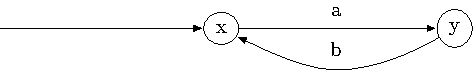
\includegraphics[width=0.3\textwidth]{automata/function/function.tikz}
  \caption{State Transition Diagram}
  \label{fig:functionDiagram}
\end{figure}
Now, for a more complex example, from \cite{cassandras2009introduction}:

\begin{example}[Simple Automaton] ~\\
  \label{ex:simpleAutomaton}
  Let $\Sigma = \{a,b,g\}$, $X = \{x,y,z\}$ and the following transition
  functions \citep{cassandras2009introduction}:
  \begin{align*}
   f(x,a)&=x&f(x,g)&=z\\
   f(y,a)&=x&f(y,b)&=y\\
   f(z,b)&=z&f(z,a)&=f(z,g)=y\\
 \end{align*}
\end{example}
We can represent this automaton with the diagram of \autoref{fig:diagramExapleAutomata}
\begin{figure}[H]
  \centering
  \includegraphics[width=0.5\textwidth]{automata/example/example.tikz}
  % \includetikzfigure[width=0.5\textwidth]{automata/example/example}
  \caption{Diagram representing the automaton from example \ref{ex:simpleAutomaton}}
  \label{fig:diagramExapleAutomata}
\end{figure}
We can also mark states that have some special meaning, as for instance, a final
state. In this work, as in \cite{cassandras2009introduction}, the marked states are identified by double circles.

  
Now a deterministic Automaton can be defined.
\begin{definition}[Deterministic Automaton]
  \label{def:DeterministicAutomaton}~\\
  A Deterministic Automaton, denoted by G, is a five-tuple
  \[ G = (X,\Sigma,f, x_0,X_m)\] where:

  \indent X is the set of \textbf{states} \\
  \indent $\Sigma$ is the finite set of \textbf{events} associated with G\\
  \indent $f: X \times \Sigma \rightarrow X$ is the \textbf{transition function}  \\
  \indent $x_0$ is the \textbf{initial state} \\
  \indent $X_m \subseteq X $ is the set of \textbf{marked states}

\end{definition}

\subsection{Petri Nets}
\label{sec:petriNets}
Another kind of representation of languages are Petri nets, whose concept was created by C.A.Petri
in the early 1960s. Differently from the automata representation, Petri nets are bipartite graphs, formed by nodes
called \emph{places} and \emph{transitions}.
Transitions represent the events that drive the system, and places represent the
conditions for these events to happen. The mechanism to represent the fulfilment
of the conditions
is named marking. A Petri net is built over three basic concepts, the petri net
graph\slash structure, its marking and firing transitions.
The next subsections will be based on \cite{david2005discrete} and \cite{cassandras2009introduction}.

\subsubsection{Petri Net Graph}
\label{sec:petrinetGraph}
Arcs are used to connect
nodes and have arrowheads to identify the direction. All arcs must have exclusively one node at each end, that means
no arc is used to identify the initial state of a Petri net. A Petri net is
bipartite graph, which means that places can only connect to transitions and vice
versa. In this work, as in \cite{david2005discrete} places are represented by
circles and transitions by bars, as shown in \Autoref{fig:componentsPetriNet}. 
\begin{figure}[H]
  \centering
  \begin{subfigure}[t]{0.45\textwidth}
  \centering
  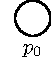
\includegraphics{petriNet/net/place.tikz}
  % \includetikzfigure[width=0.5\textwidth]{automata/example/example}
  \caption{A place.}
\end{subfigure}
~
\begin{subfigure}[t]{0.5\textwidth}
  \centering
  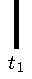
\includegraphics{petriNet/net/transition.tikz}
  % \includetikzfigure[width=0.5\textwidth]{automata/example/example}
  \caption{A transition}
\end{subfigure}
\caption{Component nodes of a petri net.}
\label{fig:componentsPetriNet}
\end{figure}

The same way a function was created to define the transitions of states in an
automaton, two functions will be created to define the connections between places
and transitions. First we need to define the sets of places and transitions. $P$
is the set of places and $T$ the set of transitions. With these two sets, we can
then define those functions. The first one represents the arcs
from places to transitions, and is denoted as $Pre: P \times T \rightarrow
\mathbb{N}$, the second one represents the arcs that connect transitions to places, denoted
as $Post: P \times T \rightarrow \mathbb{N}$. Where $\mathbb{N}=\{0,1,2,\dots\}$
is the set of non-negative integers.

% The value $1$ is attributed to arcs that exist and $0$ to the nonexistent ones.


\begin{example}[Simple Petri Net structure] ~\\
  \label{ex:simplePetriNetStructure}
  Given $P = \{p_0,p_1\}$, $T = \{t_0,t_1,t_2\}$ and the following functions:
  \begin{align*}
   Pre(p_0,t_0)& = 0  &  Post(p_0,t_1) &= 0 & Pre(p_1,t_0) &= 0 &  Post(p_1,t_1) &= 2 \\
   Post(p_0,t_0) &= 1  &    Pre(p_0,t_2) &= 0   & Post(p_1,t_0) &= 0   & Pre(p_1,t_2) &= 1\\
   Pre(p_0,t_1) &= 1    &  Post(p_0,t_2) &= 0  &  Pre(p_1,t_1) &= 0     &Post(p_1,t_2) &= 0\\
  \end{align*}
  We can represent this Petri net structure with the diagram of \autoref{fig:simplePetriNetStructureGeneralized}
\end{example}
% \begin{figure}[H]
%   \centering
%   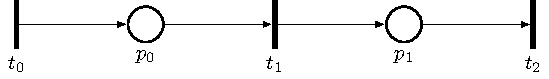
\includegraphics[width=0.5\textwidth]{petriNet/prepost/prepost.tikz}
%   % \includetikzfigure[width=0.5\textwidth]{automata/example/example}
%   \caption{Diagram representing the Petri net structure from example \ref{ex:simplePetriNetStructure}}
% \label{fig:simplePetriNetStructure}
% \end{figure}
% A drawback from the definition of this functions, is that is not possible to
% have more than an arc linking two nodes, so we can generalize them to any natural number:
% \begin{align*}
%   Pre:  P \times T \rightarrow \mathbb{N}\\
%   Post: P \times T \rightarrow \mathbb{N}
% \end{align*}
% with this new definition we can change the definition of $Post(p_1,t_1)$ from
% $0$ to $2$ resulting on the following petri net structure.
% \begin{figure}[H]
%   \centering
%   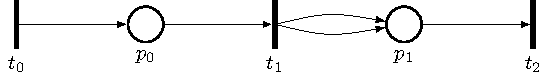
\includegraphics[width=0.5\textwidth]{petriNet/prepost/prepost2.tikz}
%   % \includetikzfigure[width=0.5\textwidth]{automata/example/example}
%   \caption{Diagram representing the petri net structure from example
%     \ref{ex:simplePetriNetStructure}, but with $Post(p_1,t_1)=2$}
% \label{fig:simplePetriNetStructureNatural}
% \end{figure}
% In order to reduce the number of arcs in a diagram, usually only one arc is
% drawn and a label is added with the value of its respective function, if it is
% greater than $1$, \autoref{fig:simplePetriNetStructureGeneralized} illustrates it:
\begin{figure}[H]
  \centering
  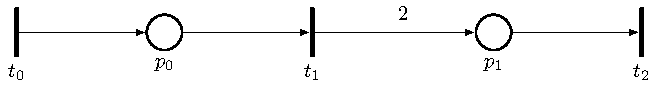
\includegraphics[width=0.5\textwidth]{petriNet/prepost/prepost3.tikz}
  % \includetikzfigure[width=0.5\textwidth]{automata/example/example}
  \caption{Diagram representing the Petri net structure from example \ref{ex:simplePetriNetStructure}}
\label{fig:simplePetriNetStructureGeneralized}
\end{figure}

\subsubsection{Marking}
\label{sec:marking}

The marking is used as the mechanism to
represent if the condition of occurrence of a determined event is met or not.
The marking also represents the state of the system. The mechanism
works as follows. Tokens can be assigned to places and the way the tokens are
distributed among places is called the marking of a Petri net graph. We can define a marking function $x :
P \rightarrow \mathbb{N}$ that denotes the number of tokens in a determined place.
In this
work, as in the majority of articles and books, the tokens will be
represented as black dots inside the places. 

\Autoref{fig:unmarked,fig:marked} show an unmarked and a marked Petri net graph, respectively.
\begin{figure}[H]
\begin{subfigure}[t]{0.45\textwidth}
  \centering
  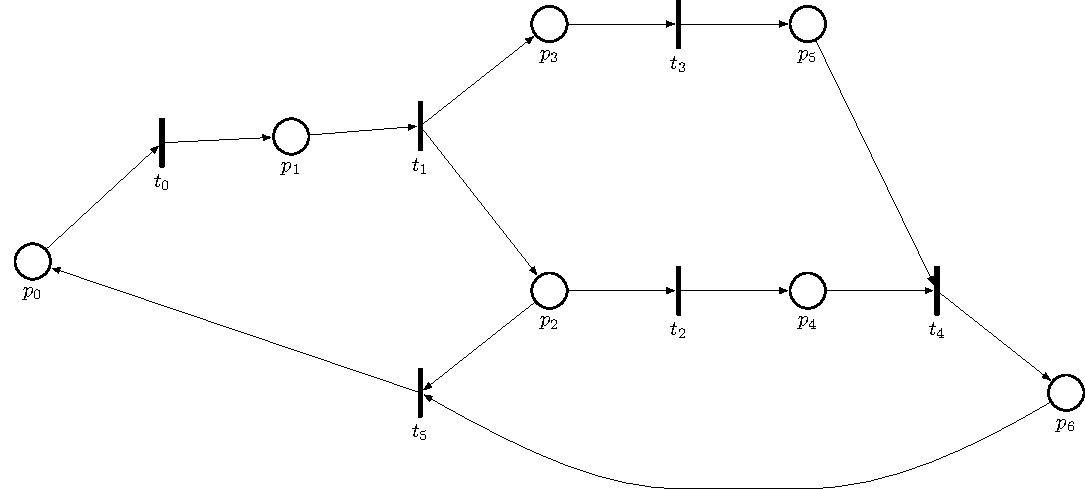
\includegraphics[width=\textwidth]{petriNet/net/unmarked.tikz}
  % \includetikzfigure[width=0.5\textwidth]{automata/example/example}
  \caption{Unmarked}
  \label{fig:unmarked}
\end{subfigure}
~
\begin{subfigure}[t]{0.45\textwidth}
  \centering
  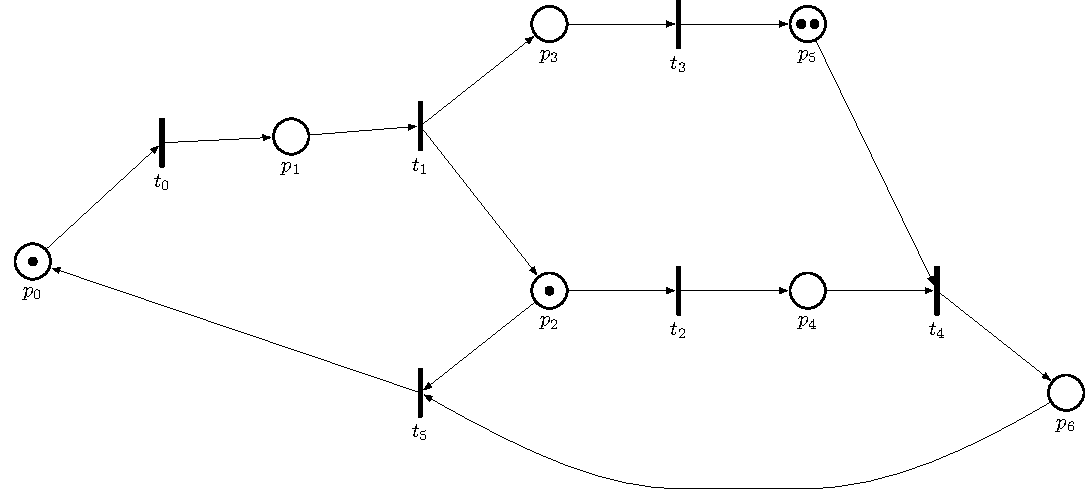
\includegraphics[width=\textwidth]{petriNet/net/marked.tikz}
  % \includetikzfigure[width=0.5\textwidth]{automata/example/example}
  \caption{Marked}
  \label{fig:marked}
\end{subfigure}
\caption{Example of unmarked and marked Petri net graphs.}
\end{figure}

The marking of a Petri net, can be represented as a
vector of the function $x$ applied on all places, for example the marking of 
\autoref{fig:marked} is the following vector.

\begin{equation*}
\mathbf{x}=\begin{bmatrix}
  x(p_0)\\
  x(p_1)\\
  x(p_2)\\
  x(p_3)\\
  x(p_4)\\
  x(p_5)\\
  x(p_6)
\end{bmatrix} =
\begin{bmatrix}
  1\\
  0\\
  1\\
  0\\
  0\\
  2\\
  0
\end{bmatrix}
\end{equation*}

 The marking of the Petri net, can be identified as the
state of the Petri net. So, different configurations of tokens mean different
states of the system, now we only need a way to change from one state to other.
\subsubsection{Firing Transitions}
\label{sec:firingTransitions}
 When an event associated with a transition $t_j$ happens and $t_j$
is enabled, $t_j$ is fired and a new marking is reached.
We can define the functions $I : T \rightarrow 2^P$ and $O : T \rightarrow 2^P$ that
describe the set of places considered as inputs and outputs of a transition: 
\begin{align*}
  I(t_j)= \{p \in P : Pre(p,t)> 0\}\\
  O(t_j)= \{p \in P : Post(p,t)> 0\}\\
\end{align*}
\begin{definition}[Enabled transition]
  \label{def:enabledTransition}~\\
  A transition is enabled if
  \[ x(p_i)\geq Pre(p_i,t_j) \text{ for all }{p_i \in I(t_j)}\]
  If $I(t_j)=\emptyset$, $t_j$ is always enabled. 
\end{definition}

And we can define the dynamic of the Petri net as follows. 

\begin{definition}[Petri net dynamics]
  \label{def:petriNetDynamics}~\\
   It is possible to define a \emph{state transition}
  function, $f : \mathbb{N}^n \times T \rightarrow \mathbb{N}^n$ , where $n$ is
  the size of the state vector $\mathbf{x}$. This function $f$ is defined for
  a transition $t_j \in T$ if and only if this transition is enabled. If
  $f(\mathbf{x},t_j)$ is defined, then we create a new state vector
  $\mathbf{x}^\prime$:

  \[ x^\prime(p_i) = x(p_i) - Pre(p_i,t_j) + Post(p_i,t_j), i=1,\dots n \]
\end{definition}
  
As an example we can take \Autoref{fig:petriNetDynamics}:
\begin{figure}[H]
  \centering
 \begin{subfigure}[t]{0.45\textwidth}
  \centering
  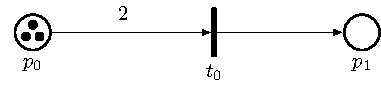
\includegraphics{petriNet/net/beforeFiring.tikz}
  % \includetikzfigure[width=0.5\textwidth]{automata/example/example}
  \caption{Before firing of $t_0$.}
  \label{fig:beforeFiring}
\end{subfigure}
~
\begin{subfigure}[t]{0.45\textwidth}
  \centering
  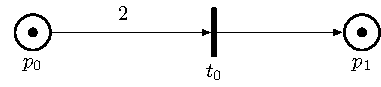
\includegraphics{petriNet/net/afterFiring.tikz}
  % \includetikzfigure[width=0.5\textwidth]{automata/example/example}
  \caption{After firing of $t_0$.}
  \label{fig:afterFiring}
\end{subfigure}
  \caption{Example of Petri net Dynamic.}
  \label{fig:petriNetDynamics}
\end{figure}
The state before firing transition $t_0$ is $\mathbf{x}=\begin{bmatrix}3&
  0\end{bmatrix}^T$ and as we see $Pre(p_0,t_0)=2$ and $Post(p_1,t_0)=1$. So, applying the Petri net dynamic, we can find the next state $\mathbf{x}^\prime=\begin{bmatrix}1&
  1\end{bmatrix}^T$.

A Petri Net is defined as follows.

\begin{definition}[Petri net]
  \label{def:petriNet}~\\
  A Petri net is defined as a five-tuple
  \[PN = (P,T,Pre,Post,\mathbf{x}_0)\]
  where: \\
  \indent $P$ is the set of \textbf{places} \\
  \indent $T$ is the set of \textbf{transitions} \\
  \indent $Pre$ is the \textbf{input incidence} function  \\
  \indent $Post$ is the \textbf{output incidence} function\\
\indent $\mathbf{x}_0$ is the initial marking of the net \\
And its dynamic is ruled by the \emph{state transition} function $f$ defined in
Definition \Autoref{def:petriNetDynamics}.

\end{definition}

To make the connection between the Petri net and the events of the system, we can
define a labeling function, $l : T^* \rightarrow \Sigma^*$ that makes the link between a
sequence of firing transitions and a sequence of events.

\begin{definition}[Labelled Petri net]
  \label{def:petriNet}~\\
  A Labelled Petri net is defined as a seven-tuple
  \[PN = (P,T,Pre,Post,\mathbf{x}_0,\Sigma,l)\]
  where: \\
  \indent $(P,T,Pre,Post,\mathbf{x}_0)$ is a Petri Net\\
  \indent $\Sigma$ is the set of \textbf{events} \\
  \indent $l$ is the \textbf{labelling} function  \\
\end{definition}

Usually, the events are represented in the Petri net graph over its respective
transition as shown in \autoref{fig:labeledPetriNet}. This system has an alphabet
$\Sigma=\{a,b\}$ and labelling functions $l(t_0)=a$ and $l(t_1)=b$.

\begin{figure}[H]
  \centering
  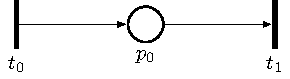
\includegraphics{petriNet/labeled/labeled.tikz}
  % \includetikzfigure[width=0.5\textwidth]{automata/example/example}
  \caption{Labeled Petri net.}
  \label{fig:labeledPetriNet}
\end{figure}

\section{Control Interpreted Petri Nets}
\label{sec:cipn}
One of the important application of Petri nets, besides modelling a system, is its
ability to model the control of a system. For this intent we use \CIPNs. It is an
extension of labelled Petri nets, in which we add actions to places, so it is
possible to change the outputs of the system, conditions to the transitions, so it
is possible to change the state of the control based on the inputs of the
system, and the ability to delay the firing transitions based on time.

\begin{definition}[Control Interpreted Petri net]
  \label{def:cipn}~\\
  A Control Interpreted Petri net is defined as a thirteen-tuple
  \[PN = (P,T,Pre,Post,\mathbf{x}_0,In,\Sigma,C,l_C,D,L_D,A,I_A)\]
  where: \\
  \indent $(P,T,Pre,Post,\mathbf{x}_0)$ is a Petri Net\\
  \indent $In$ is the \textbf{inhibitor arc} function that prevents the
  enablement of transitions \\
  \indent $\Sigma$ is the set of \textbf{events} associated to transitions \\
  \indent $C$ is the set of \textbf{conditions} associated to transitions \\
  \indent $l_C$ is the \textbf{labeling} function that associates a transition
  with events and conditions from $\Sigma$ and $C$\\
  \indent $D$ is the set of \textbf{delays} associated to timed transitions \\
  \indent $l_D$ is the \textbf{labeling} function that associates a transition with a delay from $D$ \\
  \indent $A$ is the set of \textbf{actions} associated to places \\
  \indent $l_A$ is the \textbf{labeling} function that assigns actions from $A$ to a place \\
\end{definition}
% \vspace{-0.5cm}
The definition of $In : (P \times T )\rightarrow\mathbb{N}$ is that a transition
$t_j$ is inhibited if $x(p_i)\geq In(p_i,t_j)$. Inhibitor arcs are not used in
this work but usually they are represented with an arc with a circle in one of
its ends, as shown in \autoref{fig:inhibitor}.
% \vspace{-1cm}
\begin{figure}[H]
  \centering
  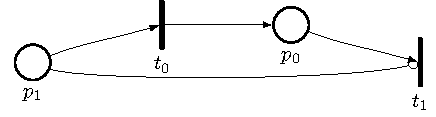
\includegraphics{petriNet/inhibitor/inhibitor.tikz}
  % \includetikzfigure[width=0.5\textwidth]{automata/example/example}
  \caption{Example of Petri net with inhibitor arc.}
  \label{fig:inhibitor}
\end{figure}
% \vspace{-1cm}
As we can see from the definition there are two labeling functions to connect 
transitions, $l_C$ and $l_D$. The $l_C$ is defined for transitions with no
firing delay and $l_D$ for transitions with firing delay.

The labeling function $l_C : T^0\rightarrow(\Sigma \times C)$ defines a pair of
event and boolean condition from $\Sigma$ and $C$ respectively. A transition
$t_i$ belonging to $T^0$ (a subset of $T$ that represents the transitions with
no time delay) has a corresponding $(event, condition)$ tuple $(\sigma_i,c_i)$
For example, take a transition $t_0$, $\Sigma =\{\sigma_0\}$ and $C=\{c_0\}$. If
a function $l_C(t_0)=(\sigma_0,c_0)$ is defined, transition $t_0$ is fired
when the condition $c_0$ is true and the event $\sigma_0$
happens, but obviously, if and only if this transition is enabled.
The transition $t_0$ is represented graphically as shown in \autoref{fig:condition}
\begin{figure}[H]
  \centering 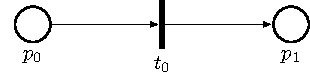
\includegraphics[width=0.3\textwidth]{petriNet/cipn/condition.tikz}
  \caption{Representation of new labeling function}
  \label{fig:condition}
\end{figure}
% \vspace{-0.4cm}
If the event is missing from the representation of the transition, it is equal
to $\lambda$, the always occurring event. And if the condition is missing, that means it is
equal to $1$, i.e. it is always $true$. If both are missing, that means the
transition will be automatically executed if it is enabled. 

On the other hand, the labeling function $l_D : T^D \rightarrow D$, defines a delay for the
transition to be fired. A timed transition $t_i \in T^D$ (a subset of T
that represents the transitions with a time delay), has a corresponding delay
$d_i$. As an example, consider a timed transition $t_1$ and $D=\{d_1\}$. Then, after the
enablement of the transition, it takes $d_1$ time units in order to be fired. In
this work, timed transitions are represented by white bars slightly larger than normal
transitions. An example of this representation we can see in \autoref{fig:timedtransition}
\begin{figure}[H]
  \centering 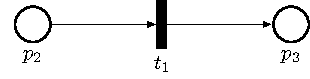
\includegraphics[width=0.3\textwidth]{petriNet/cipn/timedtransition.tikz}
  \caption{Representation of a timed transition.}
  \label{fig:timedtransition}
\end{figure}
% \vspace{-0.2cm}
Another labelling function is $l_A : P\rightarrow 2^A$,
assigning a set of actions belonging to $A$ to a place. Actions can be impulse
or continuous actions. A
continuous action happens when the marking of a place is greater than 0,
$x(p_i)>0$. An impulse action, on the other hand, happens only when the marking of
the place changes from 0 to 1. 
Actions are represented graphically as labels in places. Impulse actions are
differed by a star (*) at its end.

In \autoref{fig:actions}, a representation of a place with both kinds of actions
is presented, where $F$ is continuous and $B^\star$.
\begin{figure}[H]
  \centering 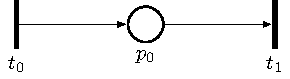
\includegraphics[width=0.3\textwidth]{petriNet/cipn/actions.tikz}
  \caption{Representation of labeling of Actions.}
  \label{fig:actions}
\end{figure}

Although these representations exist, in this work events, conditions and
action labels are suppressed from the diagrams, and tables are added to the drawings
showing the meaning of the transitions (firing events and conditions) and places
(Actions). This choice was made because the \CIPNs{}
presented in this work are very
large.

To illustrate how the tables are used to complement the information of the diagram, we give an example based on one example from \cite{david1989grafcet}.
\begin{example}[Loading of a wagon] ~\\
  \label{ex:loadingOfAWagon}
We consider the system represented by the scheme in
\autoref{fig:cipnexamplescheme}. A wagon can be moved between the points \emph{a} and
\emph{b}, using the inputs \emph{L} and \emph{R} (moving it to the left or right,
respectively). At point \emph{a} there is a button \emph{M} that can be pressed by an
operator and a limit switch called \emph{a} that is activated when the wagon is on
the left. At point \emph{b}, a homonym limit switch is placed and activated when the
wagon is on the right. There is a hopper that can
be opened when the input \emph{Open} is turned on and closed when not. If it is opened
its content is poured. There is also a
button \emph{p} that is activated when the weight applied over the plate is equal or
greater to the weight of a full wagon. 

The objective of the control is, when the wagon is in its leftmost position and
the button \emph{m} is pressed, it moves to the right, stops at \emph{b}, the hopper is
opened and the wagon is loaded. When it is completely full it moves to the left
and it stops at \emph{a} waiting to be unloaded and for a next press of \emph{m} to re-initiate
the loop. 
\end{example}


\begin{figure}[H]
  \centering \includegraphics[width=0.8\textwidth]{cipnExample/scheme.tikz}
  \caption{Example of System to be controlled by the Petri Net}
  \label{fig:cipnexamplescheme}
\end{figure}
From the description of the control it is possible to create a \CIPN{} to represent it, as the one in \autoref{fig:cipnexample}.


\begin{figure}[H]
  \centering 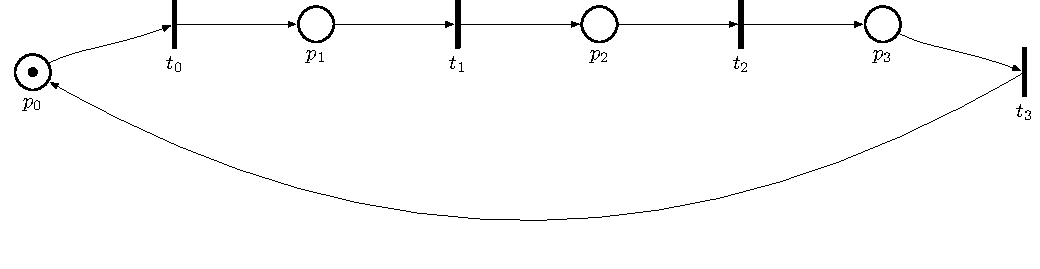
\includegraphics[width=0.8\textwidth]{cipnExample/cipn.tikz}
  \caption{Example of Control Interpreted Petri Net to control
    system in \autoref{fig:cipnexamplescheme}}
  \label{fig:cipnexample}
\end{figure}

The meaning\slash description of each place and transition is given by the
following tables:

\begin{table}[htbp]
\caption{Control Interpreted Petri Net Example Places.}
\centering
\begin{tabular}{M{5cm}M{10cm}}
Places & Meaning\\
\hline
\hyperlink{cipnExampleNet:p0m1}{\hypertarget{cipnExampleTable:p0m1}{$p_{0}$}} & System Stopped\\
\hyperlink{cipnExampleNet:p1}{\hypertarget{cipnExampleTable:p1}{$p_{1}$}} & R (Car Moving to the Right)\\
\hyperlink{cipnExampleNet:p2}{\hypertarget{cipnExampleTable:p2}{$p_{2}$}} & Open (Container Opened)\\
\hyperlink{cipnExampleNet:p3}{\hypertarget{cipnExampleTable:p3}{$p_{3}$}} & L (Car Moving to the Left)\\
\end{tabular}
\end{table}

\begin{table}[H]
\caption{Control Interpreted Petri Net Example Transitions.}
\centering
\begin{tabular}{M{5cm}M{10cm}}
Transitions & Meaning\\
\hline
\hyperlink{cipnExampleNet:t0}{\hypertarget{cipnExampleTable:t0}{$t_{0}$}} & m (filling request)\\
\hyperlink{cipnExampleNet:t1}{\hypertarget{cipnExampleTable:t1}{$t_{1}$}} & b (Right Limit Switch)\\
\hyperlink{cipnExampleNet:t2}{\hypertarget{cipnExampleTable:t2}{$t_{2}$}} & p (Car is Full)\\
\hyperlink{cipnExampleNet:t3}{\hypertarget{cipnExampleTable:t3}{$t_{3}$}} & a (Left Limit Switch)\\
\end{tabular}
\end{table}


In this work as in the usual boolean notation, when just the name of a variable is given in a table it means the
variable is equal to true, and when there is a bar in its top it is equal to
false, so they determine conditions. E.g.: $b$ and $\overline{b}$.
And when a variable is preceded by $\uparrow$ and $\downarrow$, they determine
events corresponding to its rising and falling edge.

\usetikzlibrary{arrows,shapes,circuits.plc.ladder,external}
% \pagebreak[How much [0 - 4]]
\section{Implementation of Control Interpreted Petri Nets}
\label{sec:implementPetriNets}
Once the control of a system is modeled by a \CIPN, it
is needed to implement the control in a real controller. The most used
controllers in the industry are \PLCs. The IEC 61131 standard,
defines in its third part (IEC 61131-3) the 
five languages to program \PLCs: \LD, \FBD, \ST, \IL{} and \SFC. One of the most used in the industry is \LD, because of its
resemblance with electric connections. So we are going to use \LD{} to implement the
control designed with the \CIPN.

\subsection{Ladder Logic}
\label{sec:ladder}

The ladder logic is based on two components, contacts and coils. Their terminals are
interconnected to transmit boolean signals.
Ladder comes from the resemblance between its structure (circuits formed in
parallel one above the other) and a ladder, so each circuit is called a Rung by analogy. The logic
values in a \LD{} rung
are transmitted from the left to the right of the diagram. The components let
the logic ``current'' flow from its left terminal to the right terminal
depending on some conditions, and these conditions vary from component to
component.
The rungs are executed one by one and once the very last rung is executed,
the first rung is re-executed, thus creating an infinite loop. 
 The graphical representation of the most used types of contacts and coils
can be seen in \Autoref{fig:contacts,fig:coils}

\newlength{\ladderskip}
\newlength{\ladderrungsep}

% Types of Contacts
\begin{figure}[H]
\begin{subfigure}[t]{0.45\textwidth}
  \centering \includegraphics{ladder/contactNO.tikz}
  \caption{Normally Open Contact.}
  \label{fig:contactNO}
\end{subfigure}
~
\begin{subfigure}[t]{0.45\textwidth}
  \centering \includegraphics{ladder/contactNC.tikz}
  \caption{Normally Closed Contact.}
  \label{fig:contactNC}
\end{subfigure}
\vspace{1em}

\begin{subfigure}[t]{0.45\textwidth}
  \centering \includegraphics{ladder/contactP.tikz}
  \caption{Positive Edge Contact.}
  \label{fig:contactP}
\end{subfigure}
~
\begin{subfigure}[t]{0.45\textwidth}
  \centering \includegraphics{ladder/contactN.tikz}
  \caption{Negative Edge Contact.}
  \label{fig:contactN}
\end{subfigure}

  \caption{Types of Contacts.}
  \label{fig:contacts}
\end{figure}

% Types of Coils
\begin{figure}[H]
\begin{subfigure}[t]{0.45\textwidth}
  \centering \includegraphics{ladder/coilNO.tikz}
  \caption{Coil.}
  \label{fig:contactNO}
\end{subfigure}
~
\begin{subfigure}[t]{0.45\textwidth}
  \centering \includegraphics{ladder/coilNC.tikz}
  \caption{Negated Coil.}
  \label{fig:contactNC}
\end{subfigure}
\vspace{1em}

\begin{subfigure}[t]{0.45\textwidth}
  \centering \includegraphics{ladder/coilSet.tikz}
  \caption{Set (latch) Coil.}
  \label{fig:contactP}
\end{subfigure}
~
\begin{subfigure}[t]{0.45\textwidth}
  \centering \includegraphics{ladder/coilReset.tikz}
  \caption{Reset (unlatch) Coil.}
  \label{fig:contactN}
\end{subfigure}

  \caption{Types of Coils.}
  \label{fig:coils}
\end{figure}

\subsubsection{Contacts}
Contacts represent the conditions of the ladder logic depending on inputs. These inputs can be any variable in a
\PLC, an external input (sensors of the system to be controlled), a variable stored in memory or the current
value sent to an output from the \PLC. A normally open contact
activates its right terminal (set it to $true$) if the logic value in its left terminal
is $true$ and its corresponding input is equal to $true$ 
A normally closed contact activates its right terminal if the logic value in its
left terminal is $true$ and its corresponding input is equal to $false$.
The Positive Edge contact activates its right terminal only in the instant that
its input change from logic value $false$ to $true$, if the logic value in its
left terminal is $true$. And the Negative Edge contact activates its right
terminal only in the instant that its input change from logic value $true$ to
$false$.

As we can see, positive and negative contacts can be used to represent rising ($\uparrow$)
and falling edge ($\downarrow$) events and normally open and closed contacts
to represent conditions (and their negation).

\subsubsection{Coils}

Coils, by the other side represent the actuation in outputs. These
outputs can be a variable stored in memory or the outputs
of the controller (actuators of the system to be controlled, for instance). 
A coil sets its output variable to true if the logic value of its left terminal is $true$,
and sets the output to $false$ otherwise.
A negated coil does the exact opposite, sets the output value to true if the logic
value of its left terminal is $false$ and sets it to $true$ if the logic is
$true$.

A set coil (or latch) sets its output variable to $true$ if the logic value of its
terminal is $true$ and it remains $true$ until the variable is reset.
And a reset coil (or unlatch) sets its output variable to $false$ if the logic
value of its terminal is $true$ and it remains $false$ until the variable is
set.

\subsubsection{Combinational Logic}
In boolean logic, in order to show functional completeness, it is needed to show a
complete set of connectives (a set that can create all other logic connectives
as a combination of its elements). A well-know complete set is $S=\{AND,NOT\}$,
binary conjunction and negation.
To show that the ladder logic is functional complete we need only to present how
to construct this two connectors in it.
The conjunction of two inputs, can be made using two contacts in series, as
shown in \autoref{fig:ladderSeries}.
\begin{figure}[H]
  \centering \includegraphics{ladder/series.tikz}
  \caption{And logic in a Ladder rung.}
  \label{fig:ladderSeries}
\end{figure}
In this case C will only be activated if A and B are equal to $true$. ($C=AB$)

The negation of a variable can be achieved by the use of a normally closed
contact (\autoref{fig:ladderNot}).
\begin{figure}[H]
  \centering \includegraphics{ladder/not.tikz}
  \caption{Not logic in a Ladder rung.}
  \label{fig:ladderNot}
\end{figure}
C will only by activated if A is $false$. ($C=\overline{A}$)

Although all logic connectives can be constructed with this two connectors, the
OR connector can be achieved by using contacts in parallel (\autoref{fig:ladderParallel}).
\begin{figure}[H]
  \centering \includegraphics{ladder/parallel.tikz}
  \caption{Or logic in a Ladder rung.}
  \label{fig:ladderParallel}
\end{figure}



\subsubsection{Function Blocks and extensions}
In order to increase functionality some function blocks and 
extensions to contacts were created. We can see examples of these blocks and
contacts in the next figure:

\begin{figure}[H]
   \centering
\begin{subfigure}[t]{0.45\textwidth}
  \centering \includegraphics{ladder/ctu.tikz}
  \caption{Up counter.}
  \label{fig:ctu}
\end{subfigure}
~
\begin{subfigure}[t]{0.45\textwidth}
  \centering \includegraphics{ladder/ton.tikz}
  \caption{On-delay timer.}
  \label{fig:ton}
\end{subfigure}

\begin{subfigure}[t]{0.45\textwidth}
  \centering \includegraphics{ladder/comp.tikz}
  \caption{Less or equal comparator.}
  \label{fig:comp}
\end{subfigure}
  \caption{Examples of function blocks.}
  \label{fig:functionBlocks}
\end{figure}

Up counters (\autoref{fig:ctu}) save the value of a counter in a $CV$ variable. Every raising edge
on input $CU$ it increments $CV$ value. If $CV=PV$, the logic value of output $Q$ 
is set to $0$. When the input $R$ is true $CV$ value is set to $0$ and the
output $Q$ set to false.

On-delay timers (\autoref{fig:ctu}) set a timer when input $IN$ is $true$
and save it to $ET$. If $ET=PT$, the logic value of output $Q$ is set to $true$.
But if, meanwhile the counting, the value of $IN$ returns to $false$, $ET$ is reset to
$0$.

Comparator contacts as the less or equal comparator in \autoref{fig:comp}, work
similarly to contacts, but instead of an input as a condition, there are two
inputs ($value1$ and $value2$) and the condition is a comparison between both of
them. In this case, the contact is activated once its left terminals' logic
value is $true$ and $value1\leq value2$.

Other blocks and functions can be found in the IEC 61131-3, as adders,
subtractors, communication blocks etc.

\subsection{Conversion from Control Interpreted Petri Nets to Ladder Diagram}
\label{sec:cipnToLD}

A simple method of conversion from \CIPN{} to \LD{} is presented in
\cite{moreira2013bridging}.

It consists in dividing the \CIPN{} into 4 modules:
\begin{enumerate}
\item A module of external events\\
  To create conditions to the firing of transitions based on external events
  (inputs)
\item A module of firing conditions\\
  To indicate what condition can be fired using the $Pre$, and $In$ functions, the conditions found on the
  last module and time delays (if it is a timed transition 
 )
\item A module of Petri Net dynamics\\
Uses the $Pre$ and $Post$ functions to determine the dynamics of the Petri net
\item A module of initialization\\
  It determines the initial marking of the net.
\item A module of actions\\
  It determines the places where each action is performed.
\end{enumerate}
In this work, the external events and firing conditions was combined in order to
reduce the size of the program. But every module will be described as in
\cite{moreira2013bridging}.

\subsubsection{External events}
As external events are associated with positive and negative edges of the inputs
of the system, in this module, positive and negative edge contacts are used to
detect the rising and falling edge events. The variables are stored in variables
using coils and a variable is created for each event.
For visibility's and organisation's sake a rung is used for each event,
resulting $|\Sigma|$ rungs. This module is not necessary when using Siemens
\PLCs. So it will not be used in this work.
\subsubsection{Firing Conditions}
As said in \Autoref{sec:cipn}, a transition $t_j$ fires, if it is 
enabled ($x(p_i)\geq Pre(p_i,t_j)$ for all $p_i\in I(t_j)$), not inhibited
($x(p_i)< In(p_i,t_j)$ for all $p_i\in I(t_j)$) and the conditions and events
$\sigma_jc_j$ are met or the delay $d_j$ has elapsed, depending on the kind of
transition.
As places can have multiple tokens, we can use $int$ variables to store the
number of tokens, and comparator contacts to determine if the transitions are
enabled and not inhibited.
When a place can have at most one token for all reachable markings of the
Petri net, a $boolean$ variable can be used to store the number of tokens. In this
case a normally open contact can be used to determine if there is a token
in that place.
The time delays are implemented using on-delay
timers. The state of fulfilment of the conditions is stored in variables, one
for each transition.
Similarly, for organisation's sake a rung is used for each transition, resulting
$|T|$ rungs.
\subsubsection{Petri Net Dynamics}
In this module the dynamic of the Petri net is implemented. If the condition for
the firing of a transition is fulfilled (represented by normally open contacts), adders and subtractors
can be used to represent the change in the Petri net marking. These blocks, increase and decrease the
values from the $int$ variables that represent the marking
of each place. If the capacity of the places is not greater than one, then the
marking of those places can be represented by boolean variables. Set and Reset coils can be used to
represent the marking of such places.
Again, for organisation's sake a rung is associated for each transition,
resulting $|T|$ rungs.

\subsubsection{Initialization}
The Initialization module works similarly to the dynamics module. A
initial transition is created and when this transition is fired, the marking of
the Petri net is changed to its initial marking. When the system is turned on, the condition for firing this
initial transition is true and it is disabled immediately, so this transition
can only be fired once, in the initialization phase. 

\subsubsection{Actions}
In the Action module, we use coils to act on the outputs. Depending on the type
of action and the logic of the control, set\slash reset coils or normal coils
can be used. The condition to activate\slash deactivate the output is the
presence of a token in the places where the action is performed.
This can be
achieved by comparing the numbers of tokens in a place. If the tokens of a
place is represented by an $int$ variable, we use ``greater'' or ``equal to'' comparators,
but if it is represented by a $bool$ variable, a normally open contact can be
used.
% Differently from the original article, we will use one rung per
% each action in A, resulting in $|A|$ rungs. This is made because in
% \cite{renault2017regles} it is recommended to perform an action in only one
% rung, and group the conditions using OR connectors.
% In the industry this is important in order to reduce errors and to ease the
% debugging process.
\subsubsection{Example}
An example of this conversion can be given using the same \CIPN{} from 
Example \ref{ex:loadingOfAWagon}.  The external events and firing condition
modules are grouped in the same module in this work. The converted Ladder Logic
is depicted in \autoref{fig:cipnexampleLadder}.
\begin{figure}[H]
  \centering \includegraphics{cipnExample/cipnLadder.tikz}
  \caption{Example of Control Interpreted Petri Net converted to
    Ladder.}
  \label{fig:cipnexampleLadder}
\end{figure}

\subsection{Control Interpreted Petri Net implemented in multiple PLCs}
\label{sec:multiplePlcs}
In some cases, the implementation of the control code must be carried out in
several \PLCs.
In \autoref{fig:communicationPlcPN}, it is shown an example of a \CIPN{} implemented
between 2 \PLCs.
As we can see, in \Autoref{fig:communicationPlcPN1,fig:communicationPlcPN2}
there are dotted transitions and places. In this work, we will represent as
dotted, transitions and places that are part of another section of the Petri
Net.
Those transitions and places are not represented in the same figure, 
but the arcs show the connection between the sections of the net, showing that
when connected they form a complete Petri net.
% In the digital form\footnote{Available at: \url{https://github.com/Accacio/docsTCC/raw/master/monografia.pdf}}  of this thesis it is possible to travel between
% figures that are not in the same page just by clicking in the name of the
% corresponding dotted place\slash transition.
\begin{figure}[H]
  \centering
  \begin{subfigure}[t]{0.5\textwidth}
    \center
    \includetikzfigure[width=\textwidth]{communicationPlcPN/communicationPlcPN}
    \caption{Petri Net on PLC 1.}
    \label{fig:communicationPlcPN1}
  \end{subfigure}%
  ~
  \begin{subfigure}[t]{0.5\textwidth}
    \centering
    \includetikzfigure[width=\textwidth]{communicationPlcPN/communicationPlcPN1}
    \caption{Petri Net on PLC 2.}
    \label{fig:communicationPlcPN2}
  \end{subfigure}
  \caption{Example of Petri Net implemented in 2 PLCs.}
  \label{fig:communicationPlcPN}
\end{figure}

In order to solve the problem of communication caused by the division, there are
different ways, one of them is the method shown by \cite{antunesfloriano2019sincronizacao}, where
different sections are synchronised in a distributed manner using common places.
In this work, a master\slash slave approach is used. CLP1 is considered as the
master device and CLP2 as a slave. For the master, it is created another ladder module
called ``Data Sending\slash Receiving'', divided in 2 parts.
The first part is implemented before all modules of the Ladder code, with the objective of getting all needed
variables from other \PLCs.
The second part, that is implemented after all modules of the Ladder code, with the objective of sending variables to all other \PLCs.
On the other side, the slaves have 2 additional modules, one at the beginning of
the Ladder code, called
``Prepare Received Data'' and another at the very end called ``Prepare Data to
Send''.
Those modules are created in order to avoid modification of variables in the
middle of the program cycle. Change on variables used by the
slaves \PLCs{} caused by the master during the logic can entail unexpected behaviour. 

The communication between \PLCs{} can be accomplished by using Profinet
protocol. Siemens \PLCs{} have two function blocks called ``Get'' and
``Put'', that are used to establish data transfer between two \PLCs{} using the
Profinet protocol. Tutorials on how to configure those blocks can be found on \citep{antunesfloriano2019sincronizacao,oliveira2016protocolo,rochapereira2019automacao}.
The complete implementation of the \CIPN{} depicted in
\Autoref{fig:communicationPlcPN} using \LD{} is shown in
\autoref{fig:communicationPlcPNLadder}. In
\Autoref{fig:communicationPlcPN1Ladder,fig:communicationPlcPN2Ladder}, we can see
the
conditions for transition $b0$ being transmitted from \PLC 1 to \PLC 2, and the
conditions for transition $b1$ being transmitted from \PLC 2 to PLC 1. Since the
dynamic of both conditions is divided in the two \PLCs.

  \begin{figure}[H]
    \centering
    \begin{subfigure}[t]{\textwidth}
      \begin{minipage}[b]{0.45\linewidth}
        \centering
        \resizebox{\textwidth}{!}{
          \adjustbox{trim=0 0 0 11.5cm,clip}{
            \includegraphics{communicationPlcPN/communicationPlcPNLadder.tikz}}}
      \end{minipage}
      \hspace{0.5cm}
      \begin{minipage}[b]{0.45\linewidth}
        \centering
        \resizebox{\textwidth}{!}{
           \adjustbox{trim=0 0 0 11.5cm,clip}{
           \includegraphics{communicationPlcPN/communicationPlcPNLadder.tikz}}}
      \end{minipage}
      \caption{Ladder Logic on PLC 1.}
      \label{fig:communicationPlcPN1Ladder}
    \end{subfigure}%
    \hfill
    \begin{subfigure}[t]{\textwidth}
      \begin{minipage}[b]{0.45\linewidth}
        \centering
        \resizebox{\textwidth}{!}{
          \adjustbox{trim=0 0 0 8cm,clip}{
            \includegraphics{communicationPlcPN/communicationPlcPN1Ladder.tikz}}}
      \end{minipage}
      \hspace{0.5cm}
      \begin{minipage}[b]{0.45\linewidth}
        \centering
        \resizebox{\textwidth}{!}{
          \adjustbox{trim=0 0 0 8cm,clip}{
            \includegraphics{communicationPlcPN/communicationPlcPN1Ladder.tikz}}}
      \end{minipage}
      \caption{Ladder Logic on PLC 2.}
      \label{fig:communicationPlcPN2Ladder}
    \end{subfigure}
    \caption{Example of Petri Net divided between 2 PLCs.}
    \label{fig:communicationPlcPNLadder}
  \end{figure}


% \begin{figure}[H]
%   \centering
%   \begin{subfigure}[t]{0.45\textwidth}
%     \centering
%     \includegraphics{communicationPlcPN/communicationPlcPNLadder.tikz}
%     \caption{Ladder Logic on PLC 1.}
%     \label{fig:communicationPlcPN1Ladder}
%   \end{subfigure}%
%   \hfill
%   \begin{subfigure}[t]{0.45\textwidth}
%     \centering
%     \includegraphics{communicationPlcPN/communicationPlcPN1Ladder.tikz}
%     \caption{Ladder Logic on PLC 2.}
%     \label{fig:communicationPlcPN2Ladder}
%   \end{subfigure}
%   \caption{Example of Petri Net divided between 2 PLCs.}
%   \label{fig:communicationPlcPNLadder}
% \end{figure}



The logic presented, using the master\slash slave approach, works well when
there are 2 \PLCs. When there are more \PLCs, this centralised approach
creates a single point of failure. Since master \PLC{} works as a hub, it
increases the communication delay. When there are more than two \PLCs{} it is
preferable to use a distributed approach as the one shown in
\cite{antunesfloriano2019sincronizacao}.

\section{Identification}
\label{sec:identification}

Once the control is implemented and the system is working as expected, the
identification of the system can be carried out.
In \cite{moreira2018enhanced}, a new model for \DES{} identification is proposed, called
\glsreset{DAOCT}\DAOCT. This model is created with the aim of fault detection based
on the observation of the fault free behaviour of the system, as in \cite{roth2009fdi} and \cite{klein2005fault}, but the use of path indices increases the
efficiency for fault detection when compared with the latter articles.

The fault free observation is made by acquiring the observable signals
of the system (controller inputs and outputs) for a sufficiently long
period while the system works normally. Those signals can be seen on \autoref{fig:obsSignals}.

\begin{figure}[H]
  \centering
  \begin{tikzpicture}
        % \draw[help lines,xstep=1,ystep=1] (0,0) grid (10,10);
        % \foreach \x in {0,1,...,10} { \node [anchor=north] at (\x,0) {\x}; }
        % \foreach \y in {0,1,...,10} { \node [anchor=east] at (0,\y) {\y}; }
        
        \draw[ultra thick,rounded corners] (3.5,0) rectangle (6.5,1.5);
        \draw[ultra thick,rounded corners] (0.5,2) rectangle (3.5,3.5);
        \draw[ultra thick,rounded corners] (6.5,2) rectangle (9.5,3.5);
        \draw[ultra thick,rounded corners] (3.5,4.5) rectangle (6.5,6);
        \draw (5,5.25) node {Controller};
        \draw (5,0.75) node {Plant};
        \draw (2,2.75) node {Actuators};
        \draw (8,2.75) node {Sensors};

        % actuators to plant
        \draw[->,>=stealth, very thick] (2,2) -- (2,0.75) -- (3.5,0.75);

        % controller to actuators
        \draw[->,>=stealth, very thick] (3.5,5.25) -- (2,5.25) -- (2,3.5);

        % Plant to sensors
        \draw[->,>=stealth, very thick] (6.5,0.75) -- (8,0.75) -- (8,2);

        % Sensors to controller
        \draw[->,>=stealth, very thick] (8,3.5) -- (8,5.25) -- (6.5,5.25);

        \draw[->,>=stealth, very thick] (2,4) -- (10,4);
        \draw[fill] (2,4) circle(.05);

        \draw[->,>=stealth, very thick] (8,4.5) -- (10,4.5);
        \draw[fill] (8,4.5) circle(.05);

        \draw (11,4.5) node {Observed};
        \draw (11,4.15) node {signals};

        \draw (1.5,5.75) node {Controller outputs};
        \draw (8.5,5.75) node {Controller inputs};

    \end{tikzpicture}
  \caption{Observed Signals in a closed-Loop \DES.}
    \label{fig:obsSignals}
  \end{figure}

  First, we assume the controller has $m_i$ binary inputs
  % , $i_h$, for $h=1,\dots,m_i$
  and $m_o$ binary outputs.
  % ,
  % $o_h$, for $h=1,\dots,m_o$,
  We create an Input\slash Output vector called $\mathbf{u}$ as follows:
  
\begin{equation*}
\mathbf{u}(t_1)=
\begin{bmatrix}
  i_1(t_1)&
  \dots&
  i_{m_i}(t_1)&
  o_1(t_1)&
  \dots&
  o_{m_o}(t_1)
\end{bmatrix}^T
\end{equation*}
\newcommand{\vu}{\mathbf{u}}
 Vector $\mathbf{u}(t)$ represents the status of the system in an instant
 $t$. In the \DAOCT{} model, only untimed system models are considered, thus
 the status of the system can only be modified via system events, $\sigma$.
The vector $\mathbf{u}(t)$ is also represented as $\vu_t$.
 The
 transition between status in $t_i$ and $t_j$ is represented as
 ($\vu_i,\sigma,\vu_j$).
 If a sequence of
 $l$ input\slash output vectors is observed, then the observed path of the
 system is
 $p=(\vu_1,\sigma_1,\vu_2,\sigma_2,\dots,\sigma_{l-1},\vu_l)$.
So, if we observe multiple paths in the observation process, 
multiple paths can be created
$p_i=(\vu_{i,1},\sigma_{i,1},\vu_{i,2},\sigma_{i,2},\dots,\sigma_{i,l_i-1},\vu_{i,l_i})$,
for $i=1,\dots,r$, where $r$ is the number of observed paths, and $l_i$ is the
number of vertices in each path $p_i$.

Supposing that all paths begin with the same I\slash O vector, that means, all
observations begin from the same status, it is possible to associate to each
path $p_i$ a sequence of events and a sequence of I\slash O vectors, called,
$s_i$ and $\omega_i$, defined as:
\begin{align*}
  s_i&= \sigma_{i,1}\sigma_{i,2}\dots\sigma_{i,l_i-1} \\
  \omega_i&= \vu_{i,1}\vu_{i,2}\dots\vu_{i,l_i}
\end{align*}
From the observed sequences of events $s_i$, we can define a language, called observed language, $L_{Obs}$:

\begin{equation}
  L_{Obs}:= \bigcup^r_{i=1}\overline{\{s_i\}}
\end{equation}
\begin{observation}
If any sequence $s_i$ is the prefix of another sequence $s_j$, the path $p_i$ should
be discarded, along with $s_i$ and $\omega_i$, since it does not present any new
information for the identification process.
\end{observation}
The objective of identification is to find a model that
can simulate the observed language. The language of the identified model is
called $L_{Iden}$.
We can describe the relation between these languages as $L_{Obs} \subseteq
L_{Iden}$.
In
\cite{moreira2018enhanced}, it is shown that in finite time only part of the
sequences of events that
the system can generate are observed. So, we can define the never-known language $L_{Orig}$,
the original language generated by the system.

From $L_{Orig}$ and $L_{Iden}$, another language can be defined, an exceeding
language $L_{Exc}$. The exceeding language represents the part of the identified language that is not presented in the
original language, $L_{Exc}=L_{Iden}\backslash L_{Orig}$.  The
relation between $L_{Orig}$ and $L_{Obs}$ is $L_{Obs} \subset L_{Orig}$.
And from
$L_{Orig}$ and $L_{Iden}$, $L_{OrigNI}$ can be defined. $L_{OrigNI}$
represents the part of the
original language that is not identified, $L_{OrigNI}=L_{Orig}\backslash L_{Iden}$.
The relation between all languages presented is shown in \autoref{fig:languagesVenn}.

\usetikzlibrary{patterns}
\begin{figure}[H]
  \centering
  % \sbox0{
    \includegraphics[width=0.5\textwidth]{vennDiagramLanguages.tikz}
  % }
  % \begin{minipage}{1.1\wd0}
  % \centering
   % \usebox0
  \caption{Relation between $L_{Orig}$, $L_{OrigNI}$,
    $L_{Obs}$, $L_{Exc}$ and $L_{Iden}$}.
  
  \label{fig:languagesVenn}
 % \end{minipage}
\end{figure}
As $L_{Exc}$ represents the part of the identified language that is not in
the original language, some faulty sequences will not be detected, as they are
part of the identified language. So in order to reduce the number of these non
detected faults, $L_{Exc}$ should have a cardinality as close to $0$ as 
possible.
% Reducing the cardinality of $L_{Exc}$ is possible by creating identification models that generate smaller $L_{Exc}$.

As $L_{OrigNI}$ represents the part of the original system that is not
identified, some sequences in the fault-free behaviour of the
system will be detected as faults, generating false alarms. $L_{OrigNI}$ must
also be reduced, so the false alarms generated are reduced. As the original
language of the system is never-known, it is very difficult to estimate if
$L_{OrigNI}$ is small or not. \cite{klein2005fault} show that if a system is
observed for a sufficiently long time, there exists a number $n_0\in \mathbb{N}$
such that $L_{Orig}^{\leq n_0}\backslash L_{Obs}^{\leq n_0}\approx \emptyset$,
where $L_{Orig}^{\leq n_0}$ and $L_{Obs}^{\leq n_0}$ denote the languages formed
of all sequences of events of length smaller than or equal to $n_0$ of
$L_{Orig}$ and $L_{Orig}$, respectively. Since $L_{Obs}\subseteq L_{Iden}$, $L_{OrigNI}^{\leq
  n_0}$ is also approximately the empty set.

In this work we assume that all
sequences of events that have length $n_0+1$ were observed, thus
$L_{OrigNI}^{\leq n_0}=\emptyset$.
Thus, the identified model must reduce the language $L_{Exc}^{\leq n_0}$.
% Thus, the remaining identification problem is reducing the language
% $L_{Exc}^{\leq n_0}$ and consequentially $L_{Exc}$.
\newpage
\subsection{Deterministic Automaton
  with Outputs and Conditional Transitions}
In this subsection the modified automaton model proposed by
\cite{moreira2018enhanced} is explained and the algorithm to construct it
by the observed paths $p_i$ is described. 
\begin{definition}[DAOCT]
  \label{def:daoct}~\\
  A Deterministic Automaton
  with Outputs and Conditional Transitions, denoted by DAOCT, is a nine-tuple
  \[ DAOCT = (X,\Sigma,\Omega,f,\lambda,R,\theta, x_0,X_f)\] where:

  \indent X is the set of \textbf{states} \\
  \indent $\Sigma$ is the finite set of \textbf{events}\\
  \indent $\Omega \subset \mathbb{N}_1^{m_i+m_o} $ is the set of \textbf{I/O vectors}\\
  \indent $f:  X \times \Sigma^\star \rightarrow X$ is the \textbf{deterministic transition} function  \\
  \indent $\lambda : X \rightarrow \Omega$ is the \textbf{state output} function \\
  \indent $R = {1,2,\dots,r}$ is the set of \textbf{path indices} \\
  \indent $\theta : X \times \Sigma \rightarrow 2^R$ is the \textbf{path
    estimation} function \\
  \indent $x_0$ is the \textbf{initial state} \\
  \indent $X_f \subseteq X $ is the set of \textbf{final states}
\end{definition}

The sets of events and I\slash O vectors of each path $p_i$ are denoted by $\Sigma_i$
and $\Omega_i$. Thus, $\Sigma$ and $\Omega$ can be calculated by the union of
these sets: $\Sigma=\bigcup_{i=1}^r\Sigma_i$ and
$\Omega=\bigcup_{i=1}^r\Omega_i$.
The states of the model are obtained from the vertices of the paths $p_i$, the I\slash O vectors.
Each vertex is chosen as a new state.
% But depending on the system, the vertices can be repeated in different paths and even in the same path, so a kind of memory of the past I\slash O vectors can be interesting to differentiate them, that means, taking them as different status of the system.
In some systems, certain I\slash O vectors are repeated in the same path, but with different preceding vectors.
In order to differentiate these vectors, its preceding vectors are stored in a sequence of I\slash O vectors.
% This kind of memory is presented on the form of a sequence of I\slash O vectors that stores a certain number of the past ones.
To determine the number of vectors stored in this sequence a free parameter $k$ is used. 
The modified paths created by substituting the vertices for these sequences of I\slash O vectors are denoted $p_i^k$ and are defined as follows:
\begin{equation}
  \label{eq:modifiedPath}
 p_i^k= (y_{i,1},\sigma_{i,1},y_{i,2},\sigma_{i,2},\dots,\sigma_{i,l_1-1},y_{i,l_i}) 
\end{equation}
where 
\begin{equation}
  \label{eq:modifiedPathb}
y_{i,j}=\begin{cases}
    (\vu_{i,j-k+1},\dots,\vu_{i,j}),& \quad \text{if } k\leq j\leq l_i\\
    (\vu_{i,1},\dots,\vu_{i,j}),  & \quad \text{if } j<k
  \end{cases}
\end{equation}
\newline
\begin{observation}
Depending on the choice of the value of $k$, some characteristics can be
observed on $p_i^k$. For instance, if $k=1$, $p_i^k=p_i$. And if $k$ is equal to
the larger $l_i$, then all $y_{i,l_i}$ are composed of all vertices of its
corresponding path $p_i$.
\end{observation}

\setlength\arraycolsep{2pt}
As an example of the computation of the paths $p_i^k$, let us consider the following
paths, \citep{moreira2018enhanced}:
\begin{align*}
  p_1&= \left(\colvec{1\\0\\0},a,\colvec{1\\1\\0},b,\colvec{0\\1\\1},c,\colvec{0\\0\\0},d,\colvec{0\\0\\1},e,\colvec{1\\0\\0}\right) \\
  p_2&= \left(\colvec{1\\0\\0},g,\colvec{0\\0\\0},h,\colvec{1\\1\\0},b,\colvec{0\\1\\1},c,\colvec{0\\0\\0},i,\colvec{1\\0\\0},j,\colvec{0\\1\\1},l,\colvec{1\\0\\0}\right) \\
  p_3&= \left(\colvec{1\\0\\0},g,\colvec{0\\0\\0},h,\colvec{1\\1\\0},b,\colvec{0\\1\\1},i,\colvec{1\\1\\1},m,\colvec{0\\0\\0},d,\colvec{0\\0\\1},n,\colvec{1\\1\\0}\right) \\
\end{align*}
The events of each path is associated with the rising or the falling edges of
the controller signals. Event $a$ represents the rising edge of the second
controller signal, that is $a=\uparrow$2 and event $l$ the rising edge of the first
controller signal and the falling edge of the second
and third controller signals, $l=\uparrow$1$\downarrow$2$\downarrow$3.

Since $p_i^k=p_i$, for $k=1$, in order to better illustrate the
construction of $p_i^k$, $k=2$ is chosen. Using \Autoref{eq:modifiedPath,eq:modifiedPathb} we can
obtain the following modified paths: 
\begin{align*}
  p_1^2&= \left(\colvec{1\\0\\0},a,\colvec{1&1\\0&1\\0&0},b,\colvec{1&0\\1&1\\0&1},c,\colvec{0&0\\1&0\\1&0},d,\colvec{0&0\\0&0\\0&1},e,\colvec{0&1\\0&0\\1&0}\right) \\
  p_2^2&= \left(\colvec{1\\0\\0},g,\colvec{1&0\\0&0\\0&0},h,\colvec{0&1\\0&1\\0&0},b,\colvec{1&0\\1&1\\0&1},c,\colvec{0&0\\1&0\\1&0},i,\colvec{0&1\\0&0\\0&0},j,\colvec{1&0\\0&1\\0&1},l,\colvec{0&1\\1&0\\1&0}\right) \\
  p_3^2&= \left(\colvec{1\\0\\0},g,\colvec{1&0\\0&0\\0&0},h,\colvec{0&1\\0&1\\0&0},b,\colvec{1&0\\1&1\\0&1},i,\colvec{0&1\\1&1\\1&1},m,\colvec{1&0\\1&0\\1&0},d,\colvec{0&0\\0&0\\0&1},n,\colvec{0&1\\0&1\\1&0}\right) \\
\end{align*}

% As we can see, comparing the vertices from $p_i$ with the vertices from $p_i^k$,
% the number of unique vertices from the latter is greater than the number from the former.

The states of the system are obtained from these vertices. In order to
do so, the labelling function is defined, $\tilde{\lambda}:X\rightarrow \Omega^k$. Where $\Omega^k$ is
composed of all sequences of $\Omega$ of length smaller than or equal to $k$. This
function $\tilde{\lambda}$ associates a sequence of I\slash O vectors $\omega^k
\in \Omega^k$ to each state $x \in X$. Let us denote $\tilde{\lambda_l}(x)$
as the last vector of $\tilde{\lambda}(x)$.
These functions are used in the
identification algorithm of the \DAOCT{} model.

This identification algorithm, adapted from
\cite{moreira2018enhanced}, is presented in algorithm \ref{alg:identification}.


\vspace{1cm}
\begin{algorithm2e}[H]
  \caption{Identification Algorithm}\label{alg:identification}
  \KwIn {%
    Modified observed paths $p_i^k$, for i= 1,\dots,$r$ } \KwOut {%
    DAOCT =
    $($\XSet,\SigmaSet,\OmegaSet,\ffunction,\lambdafunction,\RSet,\thetafunction,\xZero,\XfSet$)$
  } \BlankLine Create an initial state $x_0$, and define $\lambda(x_0) =
  \tilde{\lambda}(x_0) = y_{1,1}$

  $X = \{ x_0\}, X_f = \emptyset, R = \emptyset$

  \For{$i = 1$ \KwTo $r$} { $R = R \cup \{ i \}$
  
    \For{$j = 1$ \KwTo $l_i - 1$} { Find the State $x \in X $ such that
      $\tilde{\lambda}(x) = y_{i,j+1}$

      \eIf{$\tilde{\lambda}(s) \neq y_{i,j+1}$ for all $ s \in X$} { Create
        state $x^\prime$ and define $\tilde{\lambda}(x^\prime) = y_{i,j+1}$

        $X = X \cup \{ x^\prime\}$

        $\lambda(x^\prime) = \tilde{\lambda_l}(x^\prime)$

      } { Find $x^\prime \in X$ such that $\tilde{\lambda}(x^\prime) =
        y_{i,j+1}$ } $f(x,\sigma_{i,j}) = x^\prime$

      Add $i$ to $\theta(x,\sigma_{i,j})$

      \If{$j = l_i - 1$} { $X_f = X_f \cup \{x^\prime\}$ } } }
\end{algorithm2e}

\vspace{1cm}

In this algorithm, each state created represents an unique vertex of the
modified paths, and the states marked as final states represent the last vertex
of each modified path. 

Using the modified paths $p_1^1,p_2^1,p_3^1$,
% that are equal to the normal paths $p_1,p_2,p_3$,
and $p_1^2,p_2^2,p_3^2$ as inputs of \Autoref{alg:identification}, two models can be identified, one for $k=1$ and another for
$k=2$.
The state transition diagrams for the identified models are represented in \Autoref{fig:examplek1,fig:examplek2} respectively. 

\begin{figure}[H]
  \centering \includegraphics[width=\textwidth]{automata/daoct/example.tikz}
  % \includetikzfigure[width=0.5\textwidth]{automata/example/example}
  \caption{State transition diagram for identified model using $k=1$.}
  \label{fig:examplek1}
\end{figure}


\begin{figure}[H]
  \centering 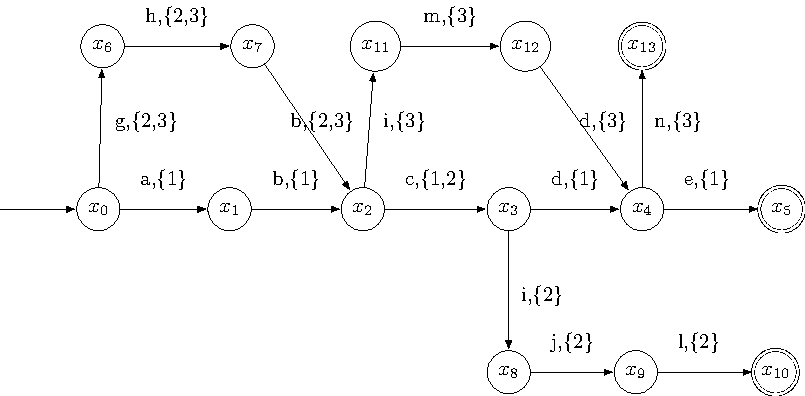
\includegraphics[width=\textwidth]{automata/daoct/examplek2.tikz}
  % \includetikzfigure[width=0.5\textwidth]{automata/example/example}
  \caption{State transition diagram for identified model using $k=2$.}
  \label{fig:examplek2}
\end{figure}

As expected, with a greater value of $k$, more states are created in the
identification process.

The path estimation function $\theta$ of each transition is represented
besides the corresponding event of that transition. That is made with the
purpose of showing the ``conditional transitions'' part of the \DAOCT{} model. A
transition is enabled and can occur if and only if all previous transitions are
associated to the same path. To summarise this in mathematical language it is
needed to expand the domain of function $\theta$ to consider sequence of events,
instead of only one event. This new estimation function will be denoted as
$\theta_s : X \times \Sigma^\star \rightarrow 2^R$, and it is defined
recursively as:
\begin{align}
  \theta_s(x,\epsilon)&=R,\nonumber\\
  \theta_s(x,s\sigma)&=
                       \begin{cases}
                         \theta_s(x,s) \cap \theta(x',\sigma),       & \quad \text{where $x^\prime = f(x,s)$, if $f(x,s\sigma)!$ }\\
                         \text{undefined, otherwise.}  &
                       \end{cases}
\end{align}
Where ! denotes \emph{is defined}.

The language generated by the identified \DAOCT{} model is given by:
\begin{align}
  L(DAOCT)&:=\{s \in \Sigma^\star : f(x_0,s)! \wedge \theta_s(x_0,s)\neq \emptyset \}
\end{align}

Using a similar logic, it is possible to define the language formed of all
subsequences of events of length $n$ generated by the identified model:
\begin{align}
  L_S^n(DAOCT)&:=\{s \in \Sigma^\star : (|s| = n)\left[\exists x_i \in X,f(x_i,s)! \wedge \theta_s(x_i,s)\neq \emptyset \right]\}
\end{align}

In order to calculate the exceeding language $L_{Exc}^{\leq n}$, another
language is presented, $L^{\leq n}(DAOCT)$, since the definition of
$L_{Exc}^{\leq n}$ is $L_{Exc}^{\leq n}=L^{\leq n}(DAOCT)\backslash
L_{Orig}^{\leq n}$.


\begin{align}
  L^{\leq n}(DAOCT)&:=\left( \bigcup_{i=0}^n L_S^i(DAOCT) \right)\cap L(DAOCT)
\end{align}
Assuming all sequences of events that have length $n_0+1$ have been
observed, then $L_{Orig}^{\leq n_0}\approx L_{Obs}^{\leq n_0}$. If $n\leq n_0$,
then $L_{Orig}^{\leq n}\approx L_{Obs}^{\leq n}$. Thus, $L_{Exc}^{\leq n}=L^{\leq n}(DAOCT)\backslash
L_{Obs}^{\leq n}$, and this formula will be used to calculate $L_{Exc}^{\leq n}$
throughout this work. 
%%% Local Variables:
%%% mode: latex
%%% TeX-master: "../monografia.tex"
%%% End:
